\documentclass[11pt,a4paper]{article}

\usepackage[utf8]{inputenc}
\usepackage[T1]{fontenc}
\usepackage[swedish]{babel}
\usepackage{amsmath,amssymb}
\usepackage{graphicx, xcolor}
\usepackage{hyperref}
\usepackage[margin=1in]{geometry}

\usepackage{subcaption}

\usepackage{amsthm}

\newtheorem{faktum}{Faktum}


\title{En budget för tillväxt?}
\author{Karl Harmenberg}
\date{\today}

\begin{document}

\maketitle

\begin{abstract}
    Presentation p� frukostseminarium med UiO.
\end{abstract}

\tableofcontents




\section{Europeisk tillväxt}

\subsection{Tillväxt i utvecklade länder}

De senaste hundra åren har karaktäriserats av en tvåprocentig tillväxt i BNP per capita för ``utvecklade'' länder så som USA och Västeuropa. Figur \ref{fig:economic_growth}, från {\color{blue}\href{https://web.stanford.edu/~chadj/facts.pdf}{Facts of Economic Growth (Jones, 2016)}}, visar tillväxten i USA.

Varför logaritm.

\begin{faktum}
    \label{faktum:us_growth}
    USA och Västeuropa har haft en tvåprocentig tillväxt i BNP per capita de senaste hundra åren.
\end{faktum}

\begin{figure}[h]
    \centering
    \begin{subfigure}[b]{0.45\textwidth}
        \centering
        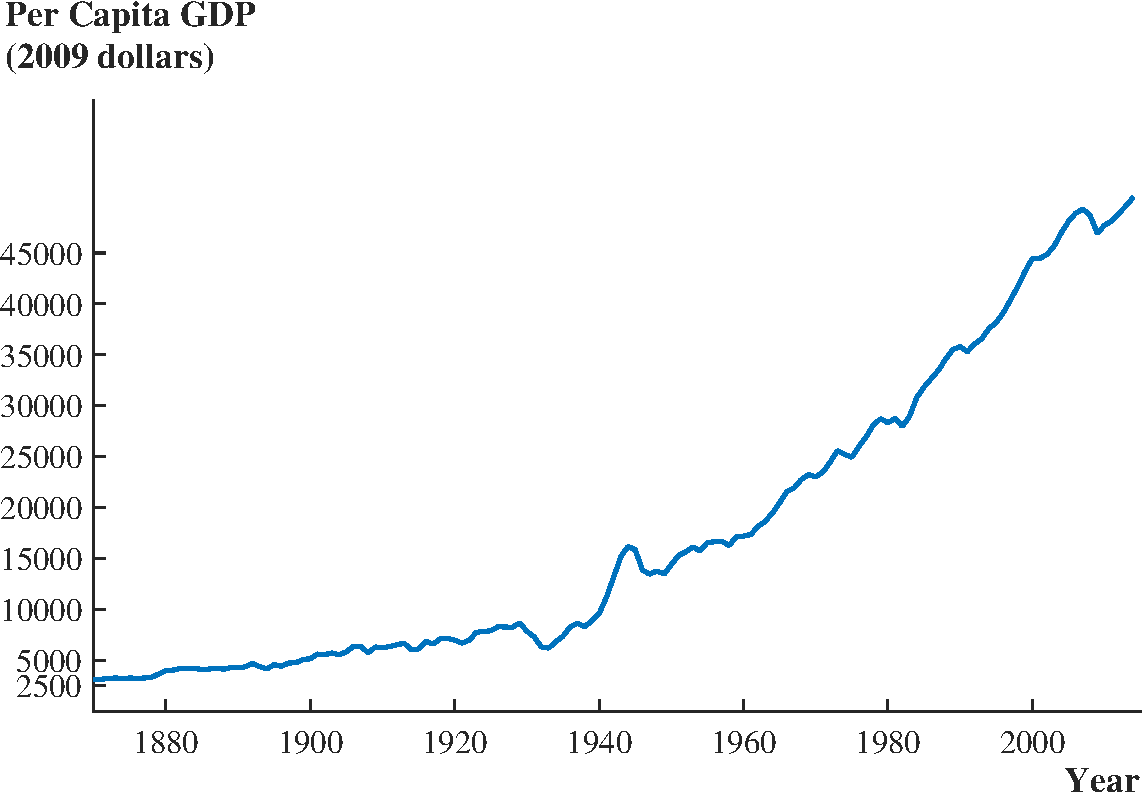
\includegraphics[width=\textwidth]{figures/uspcgdp1-crop.pdf}
        \caption{Amerikansk tillväxt.}
    \end{subfigure}
    \hfill
    \begin{subfigure}[b]{0.45\textwidth}
        \centering
        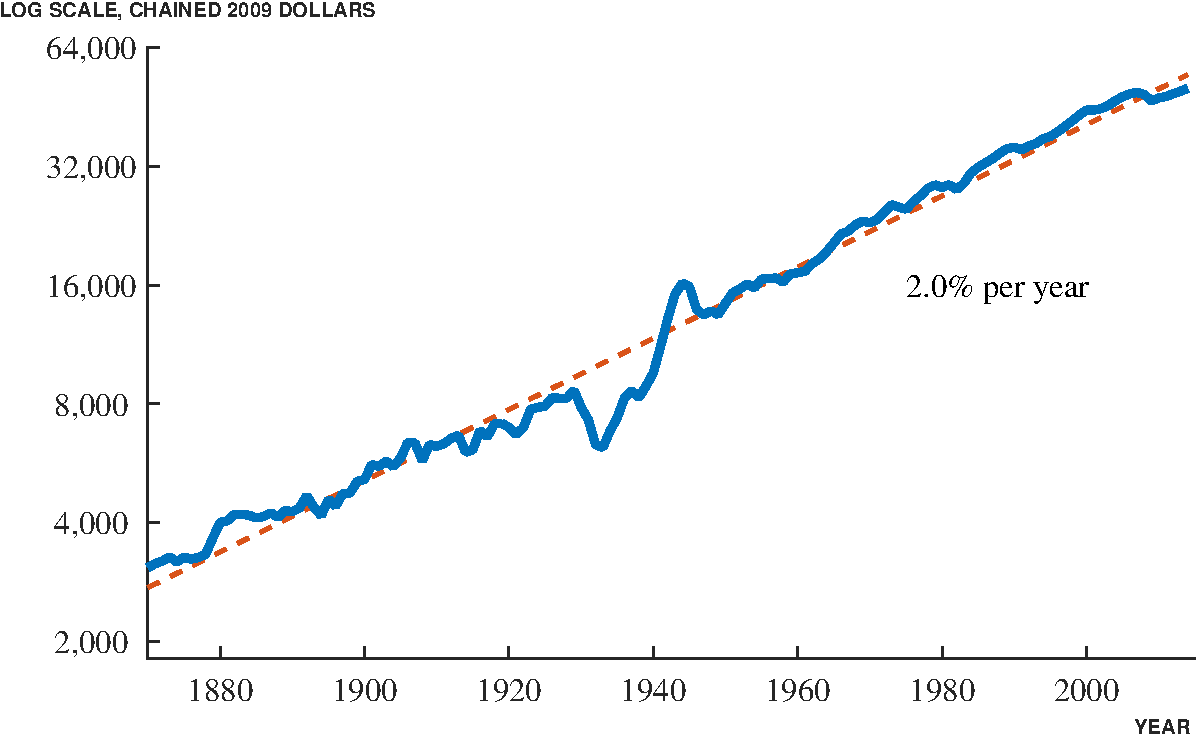
\includegraphics[width=\textwidth]{figures/uspcgdp2-crop.pdf}
        \caption{Amerikansk tillväxt, logskala.}
    \end{subfigure}
    \caption{USA, från {\color{blue}\href{https://web.stanford.edu/~chadj/facts.pdf}{Facts of Economic Growth (Jones, 2016)}}. }
    \label{fig:economic_growth}
\end{figure}

Två procent tillväxt är så klart inte en naturlag. För det första så är tillväxt ett modernt fenomen, som uppstod i samband med den industriella revolutionen. För det andra så har tillväxten under de senaste tjugo åren varit betydligt lägre, kring en procent per år.

Vad kommer tillväxten bli de kommande hundra åren? Det korta svaret är att vi inte vet. Det finns anledning att tro att de lägst hängande frukterna redan har blivit plockade, och att därför tillväxten kommer att vara lägre i framtiden. Argumentet, bland annat framfört av \cite{gordon2017}, är att 1900-talets tillväxt byggde på ett litet antal allmänt-ändamål-teknologier (``general purpose technologies''), framför allt elektricitet och förbränningsmotorer, som genererade tillväxt i alla industrier (elektriska lampor, tvättmaskiner, bilar, flyg, datorer, etc.). Utan nya genombrott och innovationer av den sorten, det vill säga som kan omvandla inte bara en liten del av en industri utan hela samhället, är det svårt att se hur tillväxten kan fortsätta i samma takt

På andra sidan i denna diskussion finns teknologioptimisterna. Datorer och internet är sådana allmänt-ändamål-teknologier, och det är möjligt att vi fortfarande befinner oss i början av den omvälvning som dessa kommer att göra i vår vardag. Vidare verkar det redan klart att artificiell intelligen i form av neurala nätverk är ytterligare en allmänt-ändamål-teknologi som kommer penetrera många industrier. Till exempel tilldelades Nobelpriset i kemi 2024 för genombrott med neurala nätverk för att förutsäga hur proteins 3D-struktur genereras av ``källkoden'' beskriven av aminosyror. Det slutgiltiga genombrottet, som mer eller mindre definitivt löste problemet att förutsäga proteins struktur, skedde så sent som 2020. Framtida tillämpningar inom till exempel läkemedelsutveckling är enorma.

\bigskip
Är hög BNP-tillväxt eftersträvansvärt? Tillväxt är inte ett mål i sig själv, snarare borde målet vara ett bra samhälle och förbättrad livskvalitet, inom ramen för vad som är ekologiskt hållbart. En del av det ökade välståndet kommer troligtvis att ``tas ut'' i form av mer fritid, inte minst som andel av livslängden. I praktiken så är ökad produktivitet, vilket egentligen bara betyder att vi finner bättre sätt att åstadkomma samma saker eller helt nya sätt att åstadkomma nya saker, en nyckel för att stadigt kunna förbättra livskvaliteten.
    
\subsection{Europeisk tillväxt}
\begin{figure}
\begin{center}
    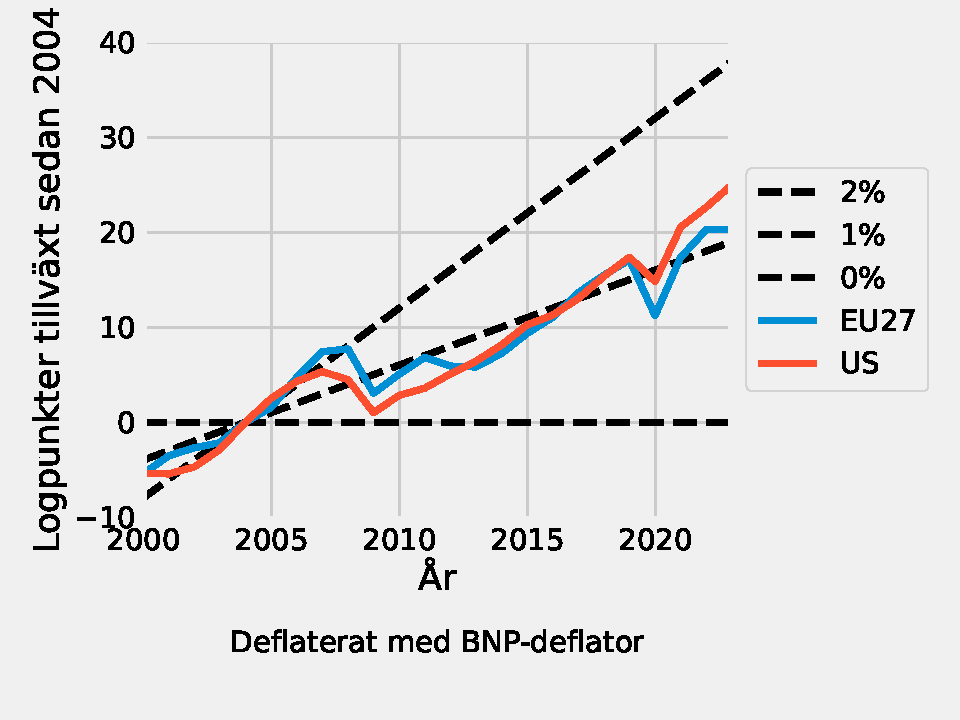
\includegraphics[width=0.7\textwidth]{figures/GDP_growth0_world.pdf}
        \end{center}
        \caption{USA och Europa har haft (väldigt) liknande tillväxt de senaste tjugo åren.}
    \label{fig:economic_growth_world}
\end{figure}

Figur \ref{fig:economic_growth_world} visar tillväxten i BNP per capita för USA och Europa de senaste tjugo åren. Genom att logaritmera så visas tillväxttakten i ``logpunkter'' vilket innebär att exponentiell tillväxt genererar en rak linje (med lutning $0.01$ motsvarande 1 procents tillväxt). Därmed så kan man med ögat skatta tillväxttakten genom att se lutningen på en linje. För bägge regionerna så normaliserar jag BNP per capita så att 2014 års nivå blir 0, man kan därmed inte använda denna graf för att jämföra nivåskillnader mellan regionerna.
I Figur \ref{fig:economic_growth_world} ser vi att tillväxten i USA och Europa har varit väldigt lik de senaste tjugo åren, omkring en procent per år. Vi sammanfattar detta i två fakta.

\begin{faktum}
    \label{faktum:recent_growth}
    De senaste tjugo åren har USA och Europa haft enprocentig tillväxt i BNP per capita.
\end{faktum}

\begin{faktum}
    \label{faktum:recent_growth_compared}
    USA och Europa har haft väldigt lik tillväxt i BNP per capita de senaste tjugo åren.
\end{faktum}

Om man har läst den omtalada Draghirapporten, skriven av Mario Draghi åt EU-kommissionen, så kan man lätt ha fått intrycket att USA har glidit ifrån Europa de senate årtiondena. I de första tre meningarna av förordet skriver Draghi:

\begin{quote}
    ``Europe has been worrying about slowing growth since the start of this century. Various strategies to raise growth
    rates have come and gone, but the trend has remained unchanged. Across different metrics, a wide gap in GDP has opened up between the EU and the US, driven mainly by a more pronounced slowdown in productivity growth in Europe.''\\
    {\color{blue}\href{https://commission.europa.eu/topics/strengthening-european-competitiveness/eu-competitiveness-looking-ahead_en}{EU Competitiveness: Looking Ahead} (Draghi, 2024)}
\end{quote}

Draghis påstående att ett brett gap har öppnat sig mellan EU och USA är helt enkelt fel, eller åtminstone väldigt missvisande. I rapporten visar Draghi att BNP har ökat betydligt snabbare i USA, men om man tittar närmare så beror detta på att USA har haft en högre tillväxt i befolkningen.\footnote{Vilket även Draghi är överens om. Han skriver: ``The gap has widened less on per capita basis as the US has seen faster population growth /.../ in PPP terms, it has risen from 31\% in 2002 to 34\% today. (s. 8)'' Se också {\color{blue}\href{https://www.piie.com/blogs/realtime-economics/2024/essential-issues-raised-not-fully-answered-draghi-report}{Blanchards och Ubides kommentar på Draghirapporten}}.} BNP per capita, vilket självklart borde vara startpunkten för en diskussion om tillväxt och välstånd, har växt i samma takt i både Europa och USA.

Även om tillväxttakten har varit lika i både Europa och USA är nivån på BNP per capita betydligt högre i USA, ungefär 30\% justerat för köpkraft. Detta gap, som har varit relativt konstant de senaste tjugo åren, är så klart betydande och europeiska politiker ska så klart fundera på om det finns konkreta grepp man kan ta för att minska gapet.


\begin{figure}
    \begin{center}
        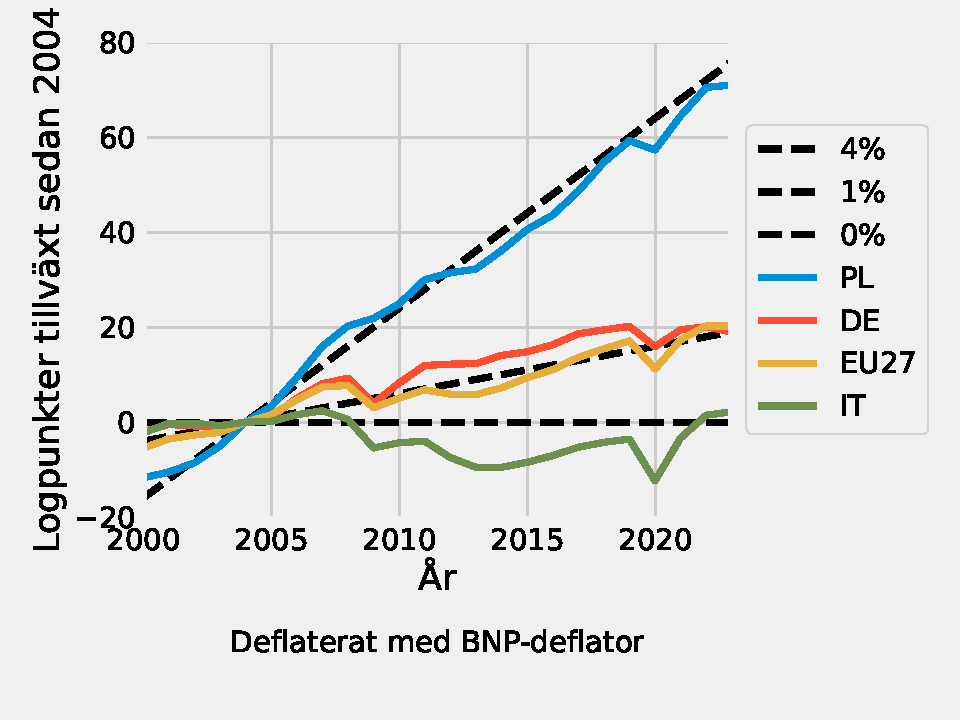
\includegraphics[width=0.7\textwidth]{figures/GDP_growth0_Europe.pdf}
        \caption{Stora variationer inom Europa. \label{fig:eu_growth_heterogeneity}}
    \end{center}
\end{figure}

Även om Europa som helhet har haft samma tillväxttakt som USA så har olika delar av Europa haft väldigt olika tillväxt. Figur \ref{fig:eu_growth_heterogeneity} visar detta. I figuren så visar jag tillväxttalen för Tyskland, Italien, Polen, och EU som helhet. Medan Italien inte har haft någon tillväxt de senaste tjugo åren så har Polen haft fyraprocentig tillväxt. I mitten, nära EU-medelvärdet, har Tyskland haft en enprocentig tillväxt.

\begin{faktum}
    \label{faktum:eu_growth_heterogeneity}
    Tillväxten varierar stort inom Europa. Östeuropa har hög tillväxt, Sydeuropa låg tillväxt, och nordeuropeiska länder har haft en tillväxt nära medelvärdet.
\end{faktum}

Östeuropas höga tillväxt är en framgångssaga.\footnote{Se {\color{blue}\href{https://cepr.org/voxeu/columns/eu-miracle-when-75-million-reached-high-income}{The EU Miracle: When 75 Million Reach High Income (Grassi, 2024)}} för en kausal ansats till att skatta effekten av EU-medlemskap på välstånd för nyare medlemsländer.} I Figur \ref{fig:eu_growth_heterogeneity_communist} visar jag tillväxten för alla nuvarande EU-medlemsländer som var kommunistländer. Tillväxttakterna är mellan två och fyra procent per år. Detta kan kontrasteras med Figur \ref{fig:eu_growth_heterogeneity_southern}, som visar tillväxten i ``PIGS''-länderna (Portugal, Italien, Grekland, Spanien). Tillväxten i dessa länder har varit låg, för Grekland till och med negativ, de senaste tjugo åren.
\begin{figure}
    \begin{center}
        \begin{subfigure}[b]{0.48\textwidth}
            \centering
            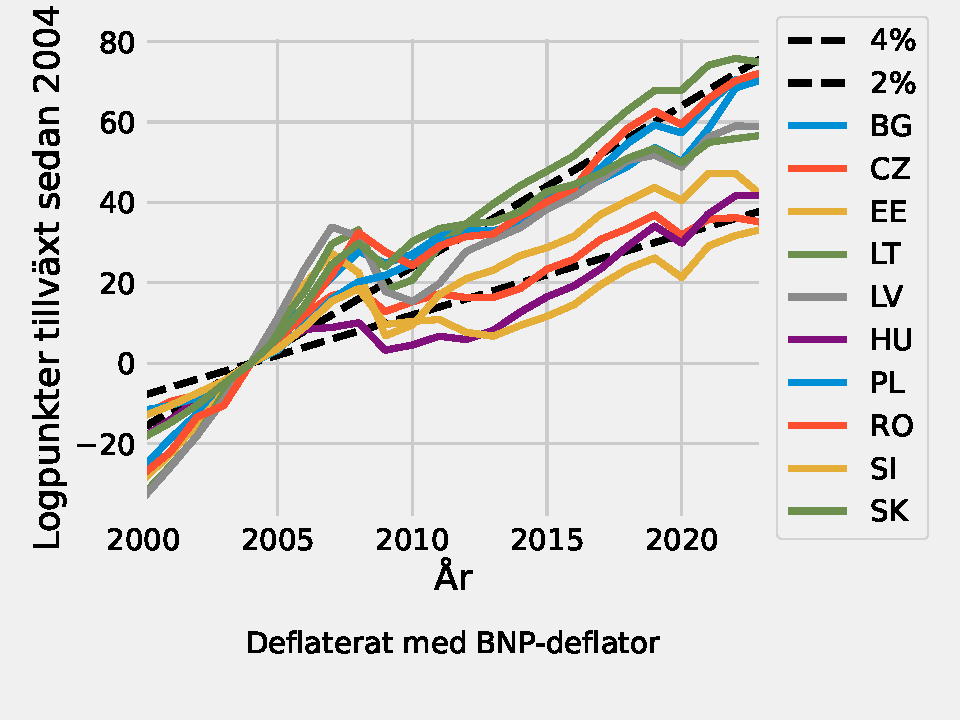
\includegraphics[width=\textwidth]{figures/GDP_growth0_Europe_former_communist.pdf}
            \caption{Hög tillväxt bland forna kommunistländer.}
            \label{fig:eu_growth_heterogeneity_communist}
        \end{subfigure}
        \hfill
        \begin{subfigure}[b]{0.48\textwidth}
            \centering
            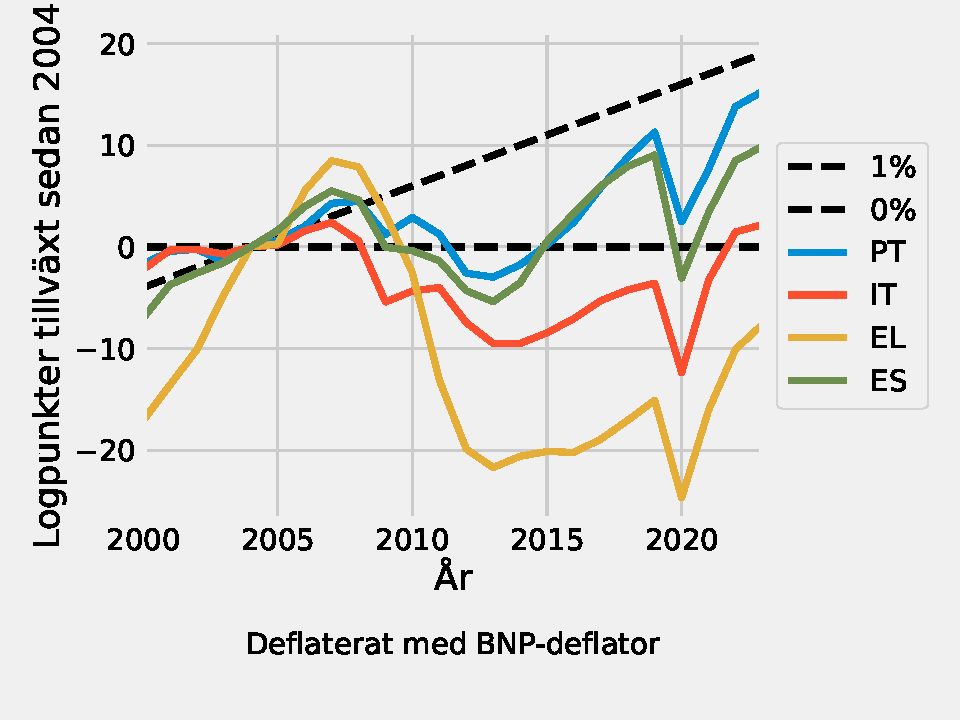
\includegraphics[width=\textwidth]{figures/GDP_growth0_PIGS.pdf}
            \caption{Låg tillväxt i Sydeuropa.}
            \label{fig:eu_growth_heterogeneity_southern}
        \end{subfigure}
        \caption{Tillväxtskillnader inom Europa}
        \label{fig:eu_growth_heterogeneity_comparison}
    \end{center}
\end{figure}
Den låga tillväxten i Sydeuropa, exemplifierat av Italien, är ett policymisslyckande. För Draghi, som italiensk byråkrat, är det naturligt att det italienska exemplet fungerar som en varning för resten av de europeiska länderna.
Italiens utveckling visar att det är långt ifrån givet att tillväxttakten i Europa kommer att hålla jämna steg med tillväxten i USA i framtiden bara för att den har gjort det de senaste tjugo åren.

\section{Norsk tillväxt}

\begin{figure}
    \begin{center}
        \begin{subfigure}[b]{0.48\textwidth}
            \centering
            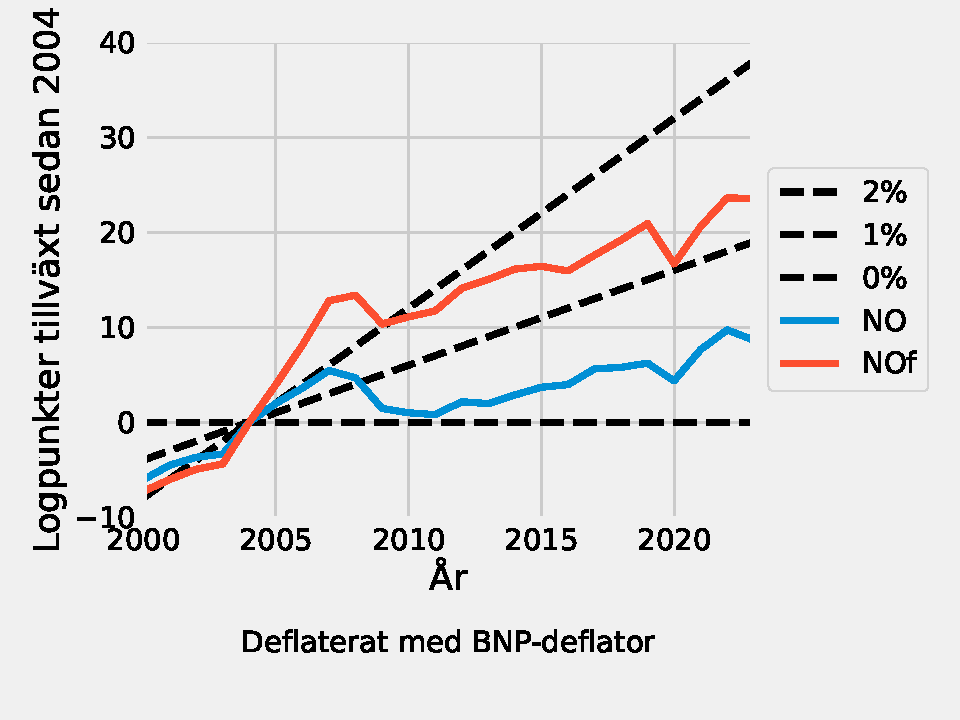
\includegraphics[width=\textwidth]{figures/GDP_growth0_NO.pdf}
            \caption{Deflaterat med BNP-deflator}
            \label{fig:norwegian_growth}
        \end{subfigure}
        \hfill
        \begin{subfigure}[b]{0.48\textwidth}
            \centering
            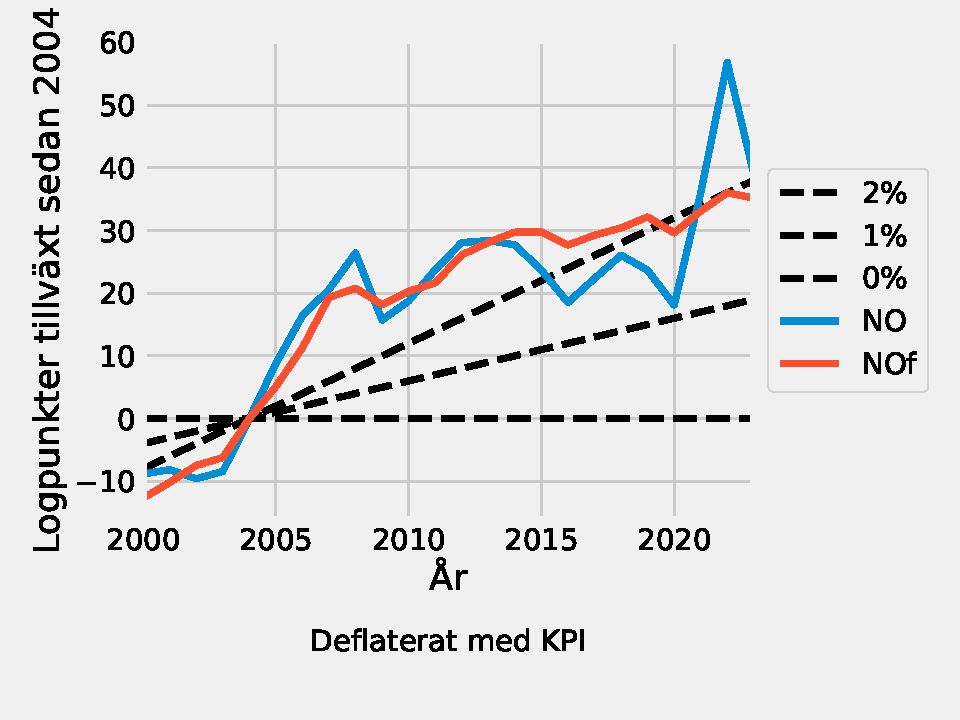
\includegraphics[width=\textwidth]{figures/GDP_growth1_NO.pdf}
            \caption{Deflaterat med KPI}
            \label{fig:norwegian_growth_kpi}
        \end{subfigure}
        \caption{Norsk tillväxt sedan 2004}
        \label{fig:norwegian_growth_comparison}
    \end{center}
\end{figure}

Låt oss nu gå vidare till vårt egna specialintresse, tillväxttakten i Norge. Figur \ref{fig:norwegian_growth} visar tillväxten i BNP per capita för Norge sedan 2004, dels för Norge inklusive oljeutvinning och dels exklusive oljeutvinnings (``Fastlandsnorge'', NOf). Tillväxttakten för Fastlandsnorge har varit drygt en procent per år, aningen högre än för Europa och USA de senaste tjugo åren, medan tillväxten inklusive oljeutvinning har varit lägre.
Denna trend kan jämföras med Perspektivmeldingens prognos för Norges tillväxt. Perspektivmeldingen 2021 prognosticerade en tillväxt på 1,1 procent per år mellan 2020 och 2060 som sammanfaller med en naiv extrapolering av trenden de senaste tjugo åren. Perspektivmeldingen 2024 reviderade den prognosen till 0,7 procent per år, vilket ligger närmare en naiv extrapolering från 2008 och framåt.

\begin{faktum}
    Fastlandsnorge har haft en tillväxt nära medelvärdet för Europa de senaste tjugo åren.
\end{faktum}

För Norge, men inte för andra länder, så är skillnaden mellan deflatering med BNP-deflator och KPI stor. Det här är en aning tekniskt, så låt mig beskriva skillnaden. BNP-deflatorn mäter priserna på allt vi producerar  medan KPI mäter priserna på det som hushållen konsumerar. För många ekonomier är skillnaden liten (och beror framför allt bytesförhållandet, ``terms of trade'', det vill säga skillnaden i export- och importpriser).

För Norge, med sin stora oljeexponering, är skillnaden stor. Real BNP deflaterat med BNP-deflatorn håller t ex oljepriset konstant och ger en lägre tillväxt de senaste tjugo åren än real BNP deflaterat med KPI. De två mäter olika saker, medan BNP deflaterat med BNP-deflatorn mäter fysisk produktion (t ex tunnor olja) så mäter KPI hur mycket mer vi kan köpa för våra inkomster.

\begin{faktum}
    Köpkrafstjusterad BNP per capita för Fastlandsnorge har haft en tvåprocentig tillväxt de senaste tjugo åren.
\end{faktum}

Norges tillväxt, deflaterat med KPI, har varit hög, omkring två procent per år. Detta gäller även Fastlandsnorge som har haft lika hög men mindre volatil KPI-deflaterad tillväxt.
Varför har Fastlandsnorge haft lika hög tillväxt som Norge inklusive oljesektorn och varför är det ett så pass stort gap mellan BNP-deflaterad tillväxt och KPI-deflaterad tillväxt? Jag vet inte, och här kan man gräva djupare, men en naturlig hypotes är att oljeindustrins efterfrågan på specifika varor och tjänster översätts i höga priser på varor och tjänster som säljs till oljesektorn. Därmed, rent bokföringsmässigt, får Fastlandsnorge en hög nominell BNP som till stor del förklaras av försäljning till oljesektorn. I och med att oljeutvinningen inte har ökat så borde det inte vara att kvantiteten efterfrågad från oljeindustrin har ökat, men på något sätt (``rents''?) har priserna ökat. Men som sagt, det här är inte något jag vet utan bara en hypotes.

\section{En budget för tillväxt?}

Så slutligen, kan vi säga något generellt om Norges tillväxtutsikter? Kan vi säga något om vilken roll politiken kan spela?
Tillväxten har varit samma i Europa, USA, Skandinavien och Norge de senaste tjugo åren. Sett från det perspektivet så har norsk politik varken varit exceptionellt bra eller dålig.
Det betyder inte att politiken inte spelar någon roll. Exempel från t ex Sydeuropa visar att länder kan hamna på en tillväxtbana långt ifrån fronten. Det vill vi undvika!

Vi behöver fortfarande en stat som möjliggör bra investeringar i humankapital, innovation och kapital, att det är möjligt att starta företag, och att Norge förblir ett attraktivt land att bo och verka i. Alla dessa punkter är nog så nära de generella målsättningar som politiska partier sätter sig.

Industripolitik är nog en del av paletten för att hålla tillväxten uppe. Som {\color{blue}\href{https://osf.io/preprints/socarxiv/gsyq4}{Juhasz, Lane och Rodrik (2024)}} skriver så är det centrala för framgångsrik industripolitik inte förmågan att ``välja vinnare'' genom att handplocka rätt industrisatsningar utan att pragmatiskt utvärdera och acceptera när industrisatsningar misslyckas (och sedan avveckla dessa satsningar på ett samhällekonomiskt effektivt sätt).\footnote{``In the presence of uncertainty, both about the effectiveness of policies and the location/magnitude of externalities, the ultimate test is not whether governments can pick `winners', but whether they have (or can develop) the ability to let `losers' go.'' (s. 6)} Jag läste i Aftenposten att tre norska batterisatsningar verkar ha misslyckats och sammantaget ha kostat staten uppemot 1 miljard norska kronor. Satsningar av den storleksordningen är ganska modesta, 200 kronor per invånare, och kan nog vara motiverade, så länge inte alltför mycket politisk prestige investeras i projekten.

Det är orealistiskt för ett litet land som Norge att vara världsledande på många fronter. Men Norge behöver inte vara det. I den mån geopolitik kräver produktion av halvledare och batterier så ska sådana åtaganden organiseras på en högre nivå än Norge (t ex EU).

Vidare så måste vi inte nödvändigtvis vara makroinnovativa för att ha fortsatt tillväxt.  Vi kan komma långt på att implementera på ett effektivt sätt redan existerande teknologier.
\href{https://www.journals.uchicago.edu/doi/abs/10.1086/693038}{Acemoglu, Robinson och Verider (2017)} gör en distinktion mellan ``cuddly capitalism'' och ``cut-throat capitalism'', där Norge är ett typexempel på det förstnämnda. Det är möjligt att våra institutioner leder till mindre innovation än amerikanska institutioner (t ex: alla techbolag är amerikanska) men det betyder inte att norsk och europeisk tillväxt är hotad. Vi kan åka snålskjuts på amerikansk entreprenöranda, och njuta av frukterna från amerikansk innovation. Ungefär som när Northug låter Calle Halfvarsson dra i front i skidspåret...

%Detta kan även gälla regionalpolitiska överväganden. En livskraftig landsbygd behöver inte betyda att varenda ort i Norge ska ha den befolkningsmängd som den har i dag.

\end{document}